\section{Arquitetura de microsserviços}

É um modelo arquitetural que tem como foco principal o baixo acoplamento dos serviços disponíveis e é altamente escalável. Ela foi criada para desacoplar as funcionalidades da arquitetura monolítica, sendo esta uma arquitetura tradicional que tem um forte acoplamento entre as classes, o que dificulta a manutenção, aumenta os custos e o tempo do projeto. Com a utilização da arquitetura de microsserviços, os serviços estarão independentes e sua manutenção pode ser realizada sem que necessite modificar a estrutura das classes de outro serviço. Esses serviços podem ser comunicados através de um barramento, como RabbitMQ e com a utilização de um protocolo de comunicação, como AMQP ou HTTP. \cite{microservices} \cite{fowler}

\subsection{Porque utilizar arquitetura de microsserviços}

Ao utilizar a arquitetura de microsserviços, torna-se fácil gerenciar as várias funcionalidades independentes do sistema. Troca de água, verificação de potencial Hidrogeniônico, controle de temperatura, controle de luminosidade e demais, são funções autônomas entre si. Em uma aplicação monolítica, qualquer alteração feita, por menor que seja, sobre um destes serviços, implica na atualização do sistema como um todo. E em caso de falhas, estas podem se propagar para demais serviços que não necessariamente estão envolvidas na atualização realizada.

Torna-se possível, também, subdividir equipes para atuarem de maneira autônoma sobre os microsserviços, sem que haja a preocupação de afetar demais subequipes. Assim, há uma distribuição de recursos (sensores, por exemplo) mais eficiente.

\subsection{Microsserviços vs SOA}

\subsubsection{Diferenças arquiteturais}

Muitos desenvolvedores realizam uma confusão por achar que a arquitetura SOA (Software Oriented-Architecture) é a mesma coisa que o estilo arquitetural de microsserviços. As duas propostas arquiteturais propõe o desenvolvimento desacoplado das funcionalidades do projeto, porém enquanto o SOA precisa de componentes que centralizam os serviços, a arquitetura de microsserviços contém os componentes descentralizados.\cite{gunter}

A imagem abaixo, ilustra essa diferença:

\begin{figure}[H]
	\centering
	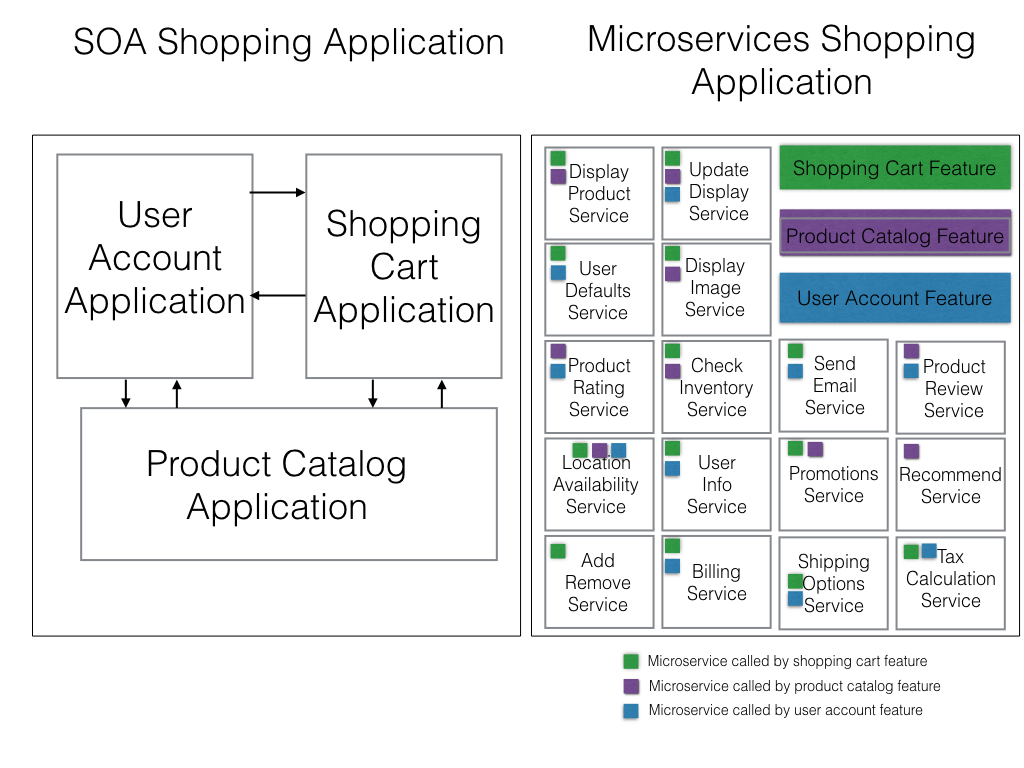
\includegraphics[width=15cm]{figuras/microsservicos.png}
	\caption{Exemplo de diferenças arquiteturais em um contexto de negócio de um sistema de supermercado.
	} \label{microsservicos}
\end{figure}

A tabela abaixo descreve as principais diferenças entre as duas arquiteturas:

\begin{table}[H]
	\centering
	\begin{tabular}{|l|l|l|}
		\hline
		\textbf{Característica}  & \textbf{Arquitetura SOA}                                                                & \textbf{\begin{tabular}[c]{@{}l@{}}Arquitetura de \\ Microsserviços\end{tabular}}                                           \\ \hline
		Tamanho do componente    & \begin{tabular}[c]{@{}l@{}}Grande parte lógica\\ do negócio\end{tabular}                & \begin{tabular}[c]{@{}l@{}}Pequeno ou pequena \\ parte da lógica do negócio\end{tabular}                                    \\ \hline
		Acoplamento              & \begin{tabular}[c]{@{}l@{}}Geralmente com \\ baixo acoplamento\end{tabular}             & \begin{tabular}[c]{@{}l@{}}Sempre com baixo \\ acoplamento\end{tabular}                                                     \\ \hline
		Estrutura organizacional & Qualquer                                                                                & \begin{tabular}[c]{@{}l@{}}Pequenas equipes \\ multifuncionais dedicadas\end{tabular}                                       \\ \hline
		Governança               & \begin{tabular}[c]{@{}l@{}}Foco na governança\\ centralizada\end{tabular}               & \begin{tabular}[c]{@{}l@{}}Foco na governança\\ descentralizada\end{tabular}                                                \\ \hline
		Objetivos                & \begin{tabular}[c]{@{}l@{}}Garante que os \\ aplicativos podem interoperar\end{tabular} & \begin{tabular}[c]{@{}l@{}}Desenvolve novos recursos \\ rapidamente para as \\ organizações em desenvolvimento\end{tabular} \\ \hline
	\end{tabular}
\caption{Principais diferenças entre arquitetura SOA e arquitetura de microsserviços.}
\label{diferencas_arquiteturais}
\end{table}

\section{Decisão arquitetural}

Baseado nas características das arquitetura SOA e microsserviços, e levando em conta as características dos stakeholders e do projeto em si,  a arquitetura de microsserviços é mais adequada pelos seguintes fatores: facilidade na integração; utilização de frameworks específicos que garante a comunicação efetiva entre os subsistemas pertinentes do projeto; pelo fato de que tanto a equipe de software como a equipe de eletrônica desenvolva em qualquer microsserviços, permitindo então a governança descentralizada que a disciplina de projeto integrador 2 disponibiliza; e, a flexibilidade e pela escalabilidade que a mesma propõe.
